\section{Application Areas}
\label{applicationareas}

One of the goals of our work is to support volume visualization for various
domains (scientific, medical), on multiple devices (workstations, virtual
reality, mobile, clusters) and on different operating systems (Linux, Mac,
Windows). This is important as VTK is used by a large user base in different
setups.  In the next few sub-sections, we have presented improvements to our
mapper for different domains and environments.

\subsection{Domains}
\label{domains}

Owing to the fact that the new mapper is built with the VTK pipeline model
(see~\Autoref{fig:pipeline}), it can be integrated into existing VTK
applications with little effort. As described
in~\Autoref{implementationdetails}, the volume mapper provides a rich
feature-set for a rendering a variety of data types. This versatility allows the
mapper to be used in diverse scientific and medical domains for volumetric
visualization. As shown in~\Autoref{fig:paraview-turbulent-combustion,
fig:tomviz-cop}, the mapper has found its way into real-world scientific
applications like ParaView~\citep{ahrens_paraview:_2005, ayachit_paraview_2015,
ayachit_paraview_2015-1} and tomviz~\citep{hanwell_tomviz_2014}. The volume
mapper can be used for
visualizing data generated from physics simulations (\Autoref{fig:supernova}),
transmission and scanning transmission electron microscopes
(\Autoref{fig:ptcu-grad}) and medical and dental CT scans
(\Autoref{fig:volume_peeling_tooth, fig:blendingmodes, fig:clipping}). 

\begin{figure}[htb]
  \begin{subfigure}[t]{0.49\columnwidth}
    \includegraphics[width=\textwidth]{SMALL-PtCu-NP-Grad.png}
    \caption{Platinum-Copper~(\ce{PtCu})
      nanoparticle \protect\citep{scott_electron_2012, miao_atomic_2016} with
      gradient opacity modulation enabled}
    \label{fig:ptcu-grad}
  \end{subfigure}\hfill%
  \begin{subfigure}[t]{0.49\columnwidth}
    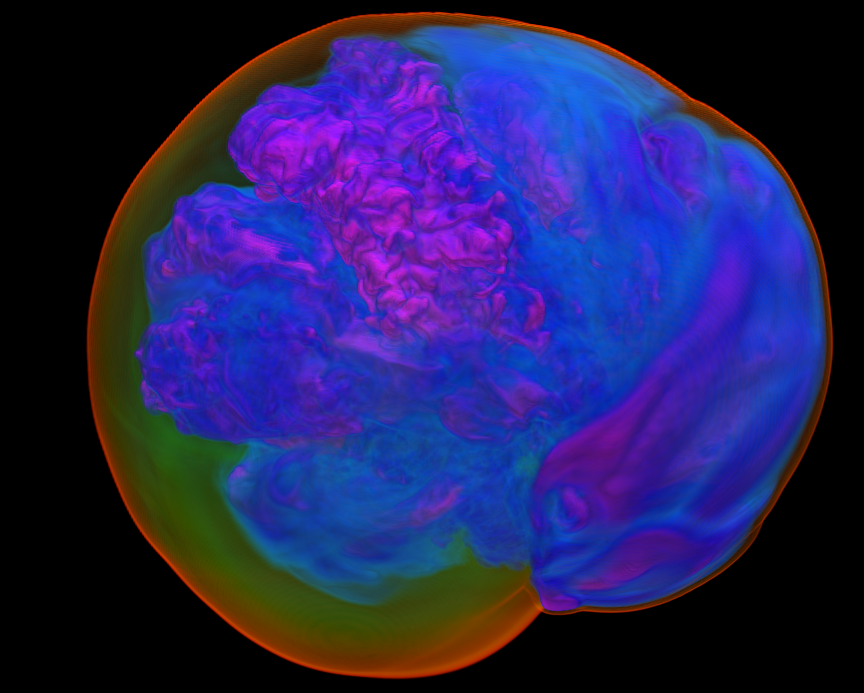
\includegraphics[width=\textwidth]{supernova-simulation.png}
    \caption{Rendering a single timestep output of the supernova modeling
      simulation~\protect\citep{blondin_pulsar_2007}}
    \label{fig:supernova}
  \end{subfigure}
  \caption{Physics and chemistry data visualization using
    the~\texttt{vtkGPUVolumeRayCastMapper}}
  \label{fig:domains}
\end{figure}

\begin{figure}[htb]
  \begin{subfigure}[t]{\columnwidth}
    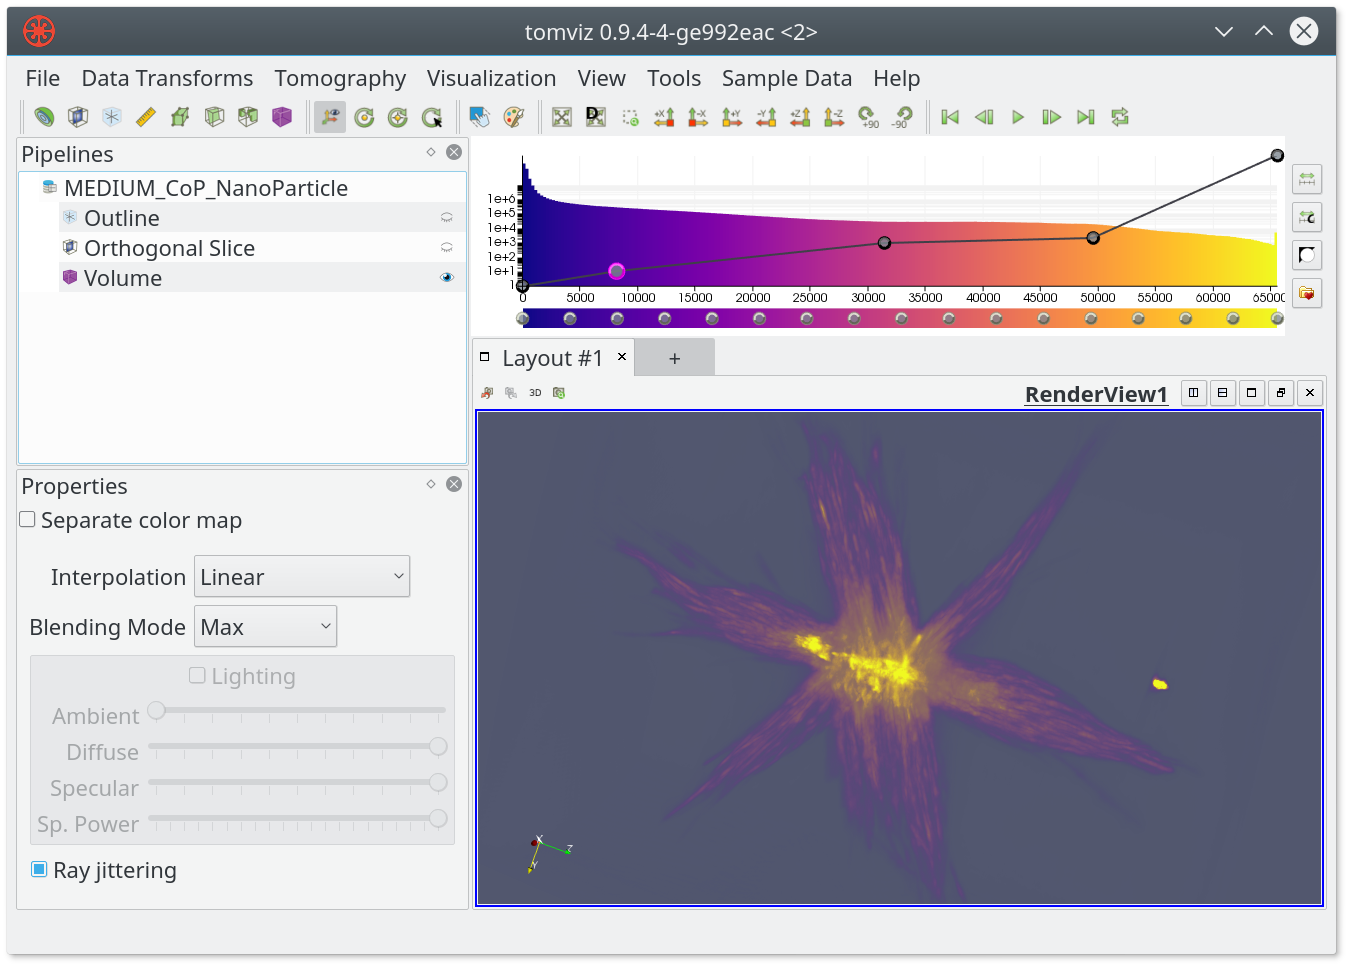
\includegraphics[width=\columnwidth]{tomviz-medium-CoP.png}
    \caption{Tomviz~\protect\citep{hanwell_tomviz_2014} rendering a
      Cobalt-Phosphorous (\ce{Co2P})
      nanoparticle~\protect\citep{levin_nanomaterial_2016}}
    \label{fig:tomviz-cop}
  \end{subfigure}
  \begin{subfigure}[t]{\columnwidth}
    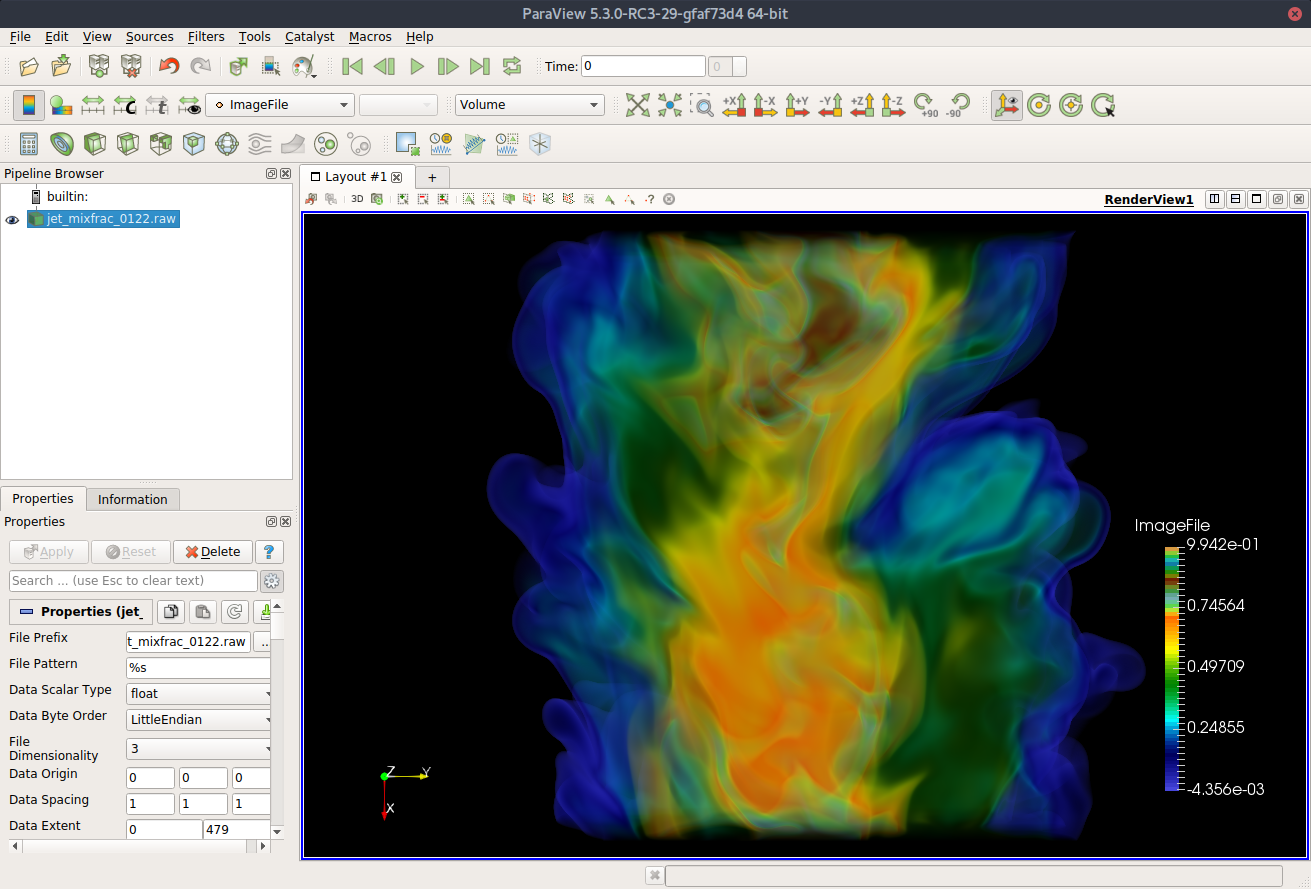
\includegraphics[width=\columnwidth]{paraview-turbulent-combustion-simulation.png}
    \caption{ParaView~\protect\citep{ahrens_paraview:_2005, ayachit_paraview_2015,
      ayachit_paraview_2015-1} rendering a single time step of a simulation of
      temporally-evolving plane jet
      flames~\protect\citep{hiroshi_akiba_visualizing_2007}}
    \label{fig:paraview-turbulent-combustion}
  \end{subfigure}
  \caption{The new~\texttt{vtkGPUVolumeRayCastMapper} has been integrated with
    existing VTK applications}
  \label{fig:application-areas}
\end{figure}

\subsection{Devices and Environments}
\label{devices-and-environments}
The new volume mapper supports rendering on most common devices including mobile
platforms.  This poses a challenge as the mapper would have to be versatile
enough to handle low computing power requirements of mobile devices and scene
composition in a multi-processor cluster environment simultaneously and still
perform at~\textit{interactive} frame rates. 

\subsubsection{Mobile Support}
\label{mobile}
The decision to use OpenGL 3 or higher enabled volume rendering to support
mobile devices (iOS and Android devices) since OpenGL ES 3.0 supports 3D textures.
However OpenGL ES does not support all of the texture format types, therefore,
new texture formats are added with compile time switches to enable or
disable them depending on whether the platform is desktop or mobile. One such
example is capturing of depth buffer since that is not yet supported on the
mobile platform.  Furthermore, as interactions on mobile devices require touch
interactions, the new rendering system added support for multi-touch events
such as using two fingers to translate, rotate, and zoom the camera. With minor
feature-set exceptions, the new volume mapper works on mobile devices enabling
developers to build sophisticated applications for the scientific community.

Various artifacts arise when rendering parallely (bricking) on a cluster.
Artifacts due to sampling, gradient computation, etc.  are seen at the edges of
each of the bricks.  To address it, our mapper ensures the entry texture
coordinate and the limit texture coordinates are correctly adjusted to, and the
ray step is scaled accordingly.

Finally, to perform consistently across various devices, our mapper uses two
critical pieces of information from VTK. First, the last frame-render time, and
second, the desired frame rate for the application. Using these two factors, the
mapper distinguishes between an~\textit{interactive} versus~\textit{still}
render and accordingly makes adjustments to the ray sampling computations to
achieve the desired frame rate. 
